\chapter{Language Server Protocol}\label{chapter:language-server-protocol}
Implementing support for features like autocomplete, refactoring, navigating to a symbol's definition, syntax highlighting, error and warning markers, or documentation on hover for a programming language is a significant effort. Traditionally this work must be repeated for each development tool, as each provides different APIs for implementing the same features.
The idea behind a Language Server is to provide the language-specific smarts inside a server that can communicate with the development tooling over a protocol that enables inter-process communication.
The Language Server Protocol was originally developed for Microsoft Visual Studio Code and is now an open standard. On 2016 June 27, Microsoft announced a collaboration with Red Hat and Codenvy to standardize the protocol's specification and it is now hosted and developed on GitHub.
The idea behind the Language Server Protocol (also called LSP from now on) is to standardize the protocol used by tools and servers to communicate, so a single Language Server can be re-used in multiple development tools, which in turn can support new languages with minimal effort.
\\\\
As can be observed in the diagram, a Language Server runs as a separate process and development tools communicate with the server using the LSP over JSON-RPC.

\begin{figure}[ht]
	\centering
	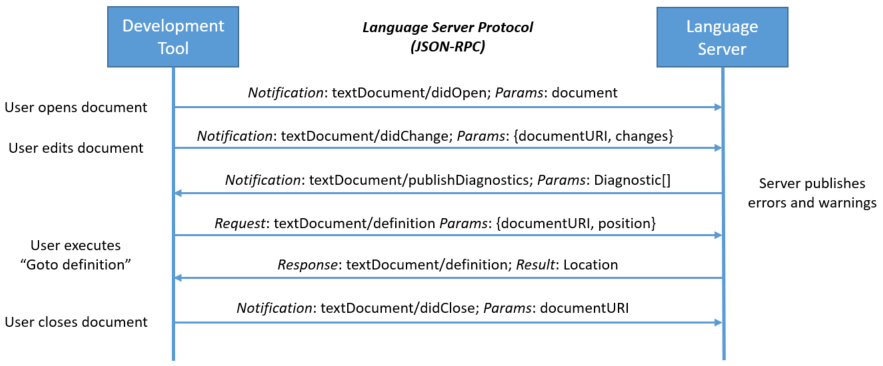
\includegraphics[width=1\textwidth]{Immagini/language-server-sequence.jpg}
	\caption{An example of communication between a tool and a Language Server through Language Server Protocol \cite{LanguageServerProtocolWebsite}}
	\label{fig:language-server-sequence}
\end{figure}

\section{The protocol}\label{sec:cap_sec_subsec}
The last version of the LSP at the time of this writing and the one that has been used in the proof-of-concept is 3.17.
The base protocol consists of a header and a content part (similar to HTTP). The header and content part are separated by a `\textbackslash r\textbackslash n'.
The header part consists of header fields which conform to the HTTP semantics. Currently the only header fields supported are Content-Length	 and Content-Type.
The content part, instead, contains the actual content of the message. This is used to send messages over JSON-RPC to describe requests, responses and notifications.

\begin{lstlisting}[caption={textDocument/didOpen notification example}, label={lst:block_struct}]
Content-Length: ...\r\n
\r\n
{
	``jsonrpc": ``2.0",
	``id": 1,
	``method": ``textDocument/didOpen",
	``params": {
		``textDocument": {
			``uri": ``file:///home/test-user/project/main.c",
			``languageId": ``c",
			``version": 1.
			``text": ``int main() { ... }"
		}
	}
}
\end{lstlisting}

\begin{lstlisting}[caption={workspace/executeCommand request example}, label={lst:block_struct}]
Content-Length: ...\r\n
\r\n
{
	``jsonrpc": ``2.0",
	``id": 1,
	``method": ``workspace/executeCommand",
	``params": {
		``command": ``trigger-analysis",
		``arguments": [``file:///home/test-user/project/main.c"]
	}
}
\end{lstlisting}

Not every Language Server can support all features defined by the protocol. LSP therefore provides \emph{capabilities}, so that both  the development tool and the Language Server can announce their supported features using capabilities at the beginning of the communication (during the ``initialize'' request). Once the capabilities of each participant in the communication are exchanged, the client and the Language Server can begin to send over requests, responses and notifications accordingly.

\section{Document Synchronization}\label{sec:cap_sec_subsec}
Each LSP client supports ``textDocument/didOpen'', ``textDocument/didChange'' and ``textDocument/didClose'' notifications. These are used by the Language Server to keep an internal synced version of the files the user is viewing. This allows the Language Server to react to changes to the file and reference specific parts of the document. For example, whenever the notification ``textDocument/didChange'' is received we can safely assume that parts of the file referenced in the notification have been changed. The LSP specification refers to three kind of document synchronization:
\begin{itemize}
  \item none, disabling all kind of document syncing;
  \item full, which means that documents are synced by always sending the full content;
  \item incremental, which means that, after sending the full content on file opening, only incremental updates to the document are sent.
\end{itemize}
In the scope of this thesis, the notification ``textDocument/didSave'' has been largely used. Below its params interface structure can be observed. 

\clearpage

\begin{lstlisting}[caption={DidSaveTextDocumentParams interface \cite{LanguageServerProtocolWebsite}}, label={lst:block_struct}]
interface DidSaveTextDocumentParams {
	/**
		* The document that was saved.
		*/
	textDocument: TextDocumentIdentifier;

	/**
		* Optional the content when saved. Depends on the includeText value
		* when the save notification was requested.
		*/
	text?: string;
}	
\end{lstlisting}

\section{Language features}\label{sec:cap_sec_subsec}
Language Features provide the actual smarts in the Language Server Protocol. Usually executed on a [text document, position] tuple, the main language feature categories are:
\begin{itemize}
	\item code comprehension features like hover or goto definition;
	\item coding features like diagnostics, code complete or code actions.
\end{itemize}
Diagnostics in particular have been the main feature used in the context of this project. In the first conceptualization of the LSP, they were something that the server could only publish to the client which were then ``owned'' by the server only, so that they were its responsibility to clear if necessary. When a file changes, it is the server's responsibility to re-compute diagnostics and push them to the client.
This approach has the advantage that for workspace-wide diagnostics the server has the freedom to compute them at a server preferred point in time. 

However, with such an approach, the server can't prioritize the computation for the file in which the user types or which are visible in the editor. Therefore, the concept of diagnostic pull requests was introduced in order to give a client more control over the documents for which diagnostics should be computed and at which point in time.
\begin{lstlisting}[caption={Diagnostic interface \cite{LanguageServerProtocolWebsite}}, label={lst:block_struct}]
export interface Diagnostic {
	/**
	 * The range at which the message applies.
	 */
	range: Range;

	/**
	 * The diagnostic's severity. Can be omitted. If omitted it is up to the
	 * client to interpret diagnostics as error, warning, info or hint.
	 */
	severity?: DiagnosticSeverity;

	/**
	 * The diagnostic's code, which might appear in the user interface.
	 */
	code?: integer | string;

	/**
	 * An optional property to describe the error code.
	 *
	 * @since 3.16.0
	 */
	codeDescription?: CodeDescription;

	/**
	 * A human-readable string describing the source of this
	 * diagnostic, e.g. `typescript' or `super lint'.
	 */
	source?: string;

	/**
	 * The diagnostic's message.
	 */
	message: string;

	/**
	 * Additional metadata about the diagnostic.
	 *
	 * @since 3.15.0
	 */
	tags?: DiagnosticTag[];

	/**
	 * An array of related diagnostic information, e.g. when symbol-names within
	 * a scope collide all definitions can be marked via this property.
	 */
	relatedInformation?: DiagnosticRelatedInformation[];

	/**
	 * A data entry field that is preserved between a
	 * `textDocument/publishDiagnostics' notification and
	 * `textDocument/codeAction' request.
	 *
	 * @since 3.16.0
	 */
	data?: unknown;
}
\end{lstlisting}
